\documentclass[a4paper, 11pt]{scrartcl}

\usepackage{graphicx}
\usepackage[ngerman]{babel}
\usepackage{emoji}
\usepackage{svg}
\usepackage{lipsum}
\usepackage{tikz}
\usepackage{todonotes}
\usepackage{caption}
\usepackage{subcaption}
\usepackage[margin=2cm]{geometry}
\usepackage{float}

\usetikzlibrary{calc, positioning, shapes}

\pagenumbering{gobble}

\newcommand{\backendcolor}{blue!40}
\newcommand{\frontendcolor}{red!40}
\newcommand{\eventcolor}{orange!40}

\newcommand{\technicaldebt}[1]{\tikz[baseline=-0.7ex]\node[scale=0.4, fill=#1, draw, circle, minimum width=1cm] () {};}
\newcommand{\technicaldebtfrontend}{\technicaldebt{\frontendcolor}}
\newcommand{\technicaldebtbackend}{\technicaldebt{\backendcolor}}

\newcommand{\feature}[1][]{Feature#1 \emoji{clipboard}}
\newcommand{\bug}[1][]{Bug#1 \emoji{beetle}}
\newcommand{\event}[1][]{Event#1 \emoji{calendar}}

\newcommand{\storypoint}{\emoji{teddy-bear}}

\newcommand{\personaharald}{Harald \emoji{old-man-medium-skin-tone}}
\newcommand{\personamathilde}{Mathilde \emoji{woman-dark-skin-tone}}
\newcommand{\personasabine}{Sabine \emoji{woman-medium-skin-tone}}
\newcommand{\personamark}{Mark \emoji{man-medium-skin-tone-curly-hair}}

\begin{document}

\setemojifont{TwemojiMozilla}

\section*{Hintergrund}

Willkommen bei der MagicSoftware GmbH. Wir freuen uns, dass ihr heute bei uns anfangt. Wie ihr wisst, bauen wir Software für die Digitalisierung des Berichtwesens. Vor einem Jahr haben wir \glqq agile\grqq\ als Arbeitsmodus eingeführt. Entsprechend werdet ihr euch bestimmt schnell eingewöhnen. Vielleicht erst einmal zu eurem Team:

\noindent\personaharald\ ist euer Teamleiter. Er war früher als Entwickler bei uns tätig, bevor er nun die Leitung des Teams übernommen hat. Entsprechend kann er euch gut bei allen Blockern unter die Arme greifen.\\
\personamathilde\ kommt aus der Quality Assurance und ist entsprechend eure Ansprechpartnerin für alles was Tests angeht.\\
\personasabine\ ist die Kundenmanagerin. Das heißt, ihr müsst euch nicht selbst mit den Kunden rumschlagen. Sie hält euch den Rücken frei. Gleichzeitig haben wir aber etwas Mitarbeiterknappheit, sodass Sabine an anderer Stelle aushelfen muss. Habt bitte etwas Nachsicht.\\
\personamark\ ist der Kunde. Ihr werdet zwar nicht direkt mit ihm in Kontakt treten, aber es ist ja auch gut zu wissen, für wen man eigentlich arbeitet.

\noindent Der Projektabschluss wird in neun Iterationen sein. Ein bisschen was ist von euren Vorgängern erledigt. Anderes wiederum ist liegen geblieben. Aber das werdet ihr schon schaffen. Viel Erfolg!

\section*{Spielelemente}

\begin{itemize}
    \item 9 Event-Karten
    \item 39 Ticket-Karten, davon:
    \begin{itemize}
        \item 27 Features
        \item 12 Bugs
    \end{itemize}
    \item 12 Wendechips für Technical Debt
    \item 20 Bärchen für Storypoints
    \item 1 Spielfeld
\end{itemize}

\subsection*{Event-Karten}

\begin{figure}[H]
    \centering
    \begin{tikzpicture}
        \node[draw, inner sep=0cm, line width = 1mm] (card) {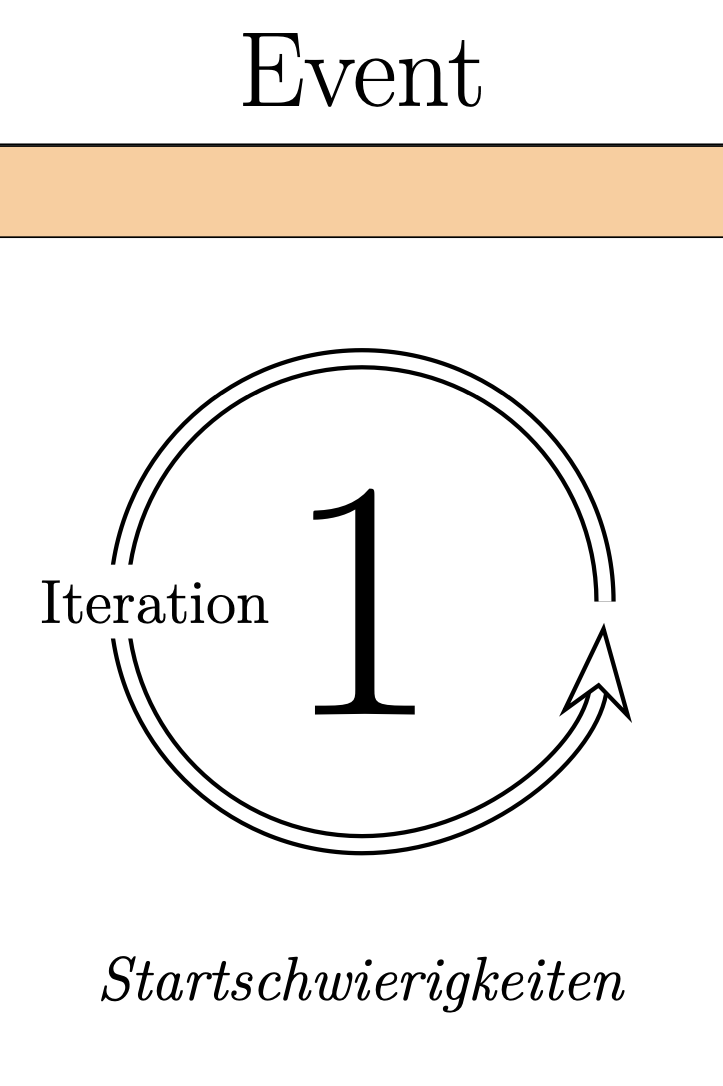
\includegraphics[width=0.3\textwidth]{images/event}};

        \node[anchor=north west, text width = 6cm] (title) at ($(card.north east) + (1cm, -0.3cm)$) {\textbf{Kartenart}: Events sind unvorhergesehene Ereignisse, die während des Projekts auftreten. Ob sie sich positiv oder negativ auswirken erfahrt ihr bei der Ausführung.};
        \draw[->, line width = 1mm, dotted] ($(title.north west) + (0mm, -2.5mm)$) -- ($(title.north west) + (-25mm, -2.5mm)$);

        \node[anchor=west, text width = 6cm] (iteration) at ($(card.east) + (1cm, -0.45cm)$) {\textbf{Kommende Iteration}. Insgesamt gibt es neun Iteration.};
        \draw[->, line width = 1mm, dotted] ($(iteration.north west) + (0mm, -2.5mm)$) -- ($(iteration.north west) + (-15mm, -2.5mm)$);

        \node[anchor=south west, text width = 6cm] (foreshadowing) at ($(card.south east) + (1cm, -0.5cm)$) {\textbf{Titel}: Gibt euch eine grobe Idee, was ihr diese Iteration zu erwarten habt.};
        \draw[->, line width = 1mm, dotted] ($(foreshadowing.north west) + (0mm, -2.5mm)$) -- ($(foreshadowing.north west) + (-15mm, -2.5mm)$);
    \end{tikzpicture}
\end{figure}

\subsection*{Tickets}

\begin{figure}[H]
    \begin{tikzpicture}
        \node[draw, inner sep=0cm, line width = 1mm, anchor=west] (bug) {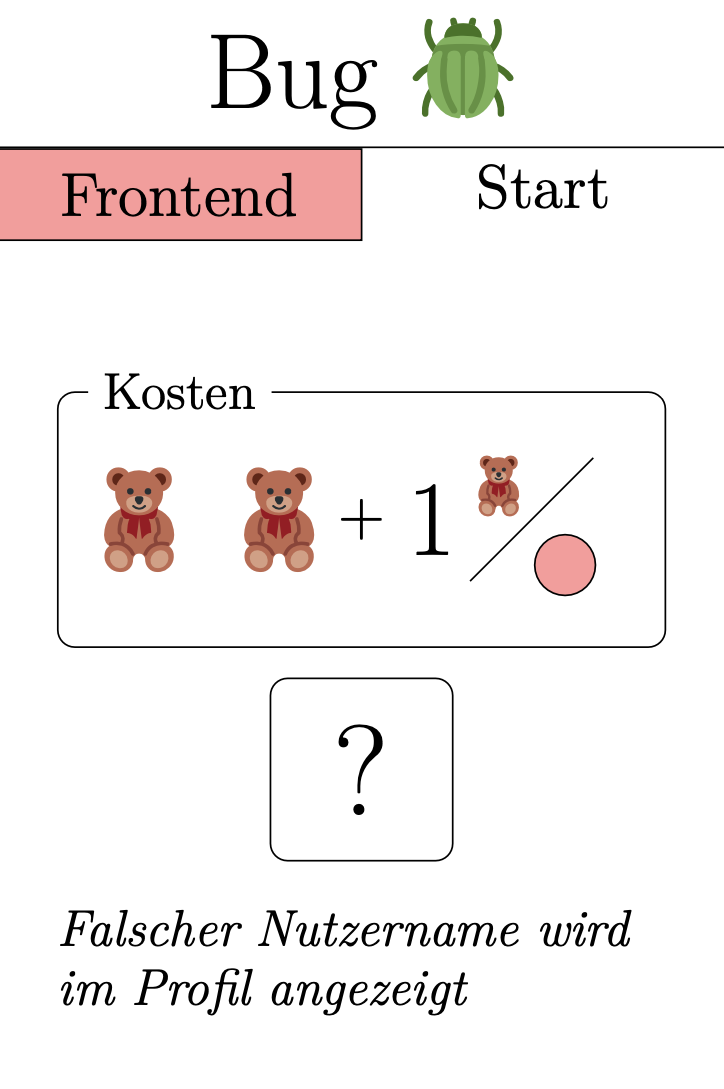
\includegraphics[width=0.3\textwidth]{images/bug}};

        \node[anchor = south, text width = 100mm] (kartenart) at ($(bug.north) + (0mm, 10mm)$) {\textbf{Kartenart}: Zeigt ob es sich um ein Feature oder einen Bug handelt. Der Unterschied zwischen den beiden ist, dass nur Features euch Punkte bringen, sie dafür aber auch Technical Debt erzeugen. Bugs tun das nicht.};
        \draw[->, line width = 1mm, dotted] (kartenart.south) -- ($(kartenart.south) + (0mm, -13mm)$);
        \node[anchor = north west, text width = 50mm] (startmarker) at ($(bug.north east) + (10mm, -2.5mm)$) {\textbf{Start-Marker (optional)}: Gibt an, ob das Ticket zu Spielbeginn im Backlog liegt.};
        \draw[->, line width = 1mm, dotted] ($(startmarker.west) + (0mm, -3.5mm)$) -- ($(startmarker.west) + (-18mm, -3.5mm)$);

        \node[anchor = west, text width = 50mm] (cost) at ($(bug.east) + (10mm, -5mm)$) {\textbf{Kosten}: Anzahl Storypoints, die ihr für das Ticket aufwenden müsst. Der feste Anteil sind die Bärchen auf der linken Seite. Oben drauf kommt ein weiterer Storypoint je Technical Debt in dem Systemteil.};
        \draw[->, line width = 1mm, dotted] ($(cost.west) + (0mm, 6mm)$) -- ($(cost.west) + (-13mm, 6mm)$);

        \node[anchor = south west, text width = 50mm] (title) at ($(bug.south east) + (10mm, 0mm)$) {\textbf{Titel}: Eine Beschreibung des abzuarbeitenden Tickets.};
        \draw[->, line width = 1mm, dotted] ($(title.north west) + (0mm, -2.5mm)$) -- ($(title.north west) + (-15mm, -2.5mm)$);

        \node[anchor = north east, text width = 50mm] (system) at ($(bug.north west) + (-10mm, -7mm)$) {\textbf{Systemteil}: Gibt an, ob das Ticket das Frontend oder das Backend betrifft.};
        \draw[->, line width = 1mm, dotted] (system.east) -- ($(system.east) + (13mm, 0mm)$);

        \node[anchor = south east, text width = 50mm] (hint) at ($(bug.south west) + (-10mm, 5mm)$) {\textbf{Effekthinweis}: Beim Abarbeiten eines Tickets führt ihr den Effekt auf der Rückseite aus. Der Effekthinweis zeigt, ob ihr einen positiven (\tikz[baseline=-1ex]\node[scale=0.4, single arrow, draw, fill=white, rotate=90, minimum height = 1cm, minimum width = 1cm] {};), negativen (\tikz[baseline=-0.5ex]\node[scale=0.4, single arrow, draw, fill=white, rotate=270, minimum width = 1cm, minimum height = 1cm] {};) oder zufälligen (?) Effekt bekommt.};
        \draw[->, line width = 1mm, dotted] (hint.east) -- ($(hint.east) + (27mm, 0mm)$);
    \end{tikzpicture}
\end{figure}

\subsection*{Technical Debt}

Technical Debt macht es schwieriger, neue Funktionalität zu bauen. Wie viel Technical Debt ihr habt wird durch die entsprechenden Tokens dargestellt. Im Frontend sehen sie so aus: \technicaldebtfrontend. Im Backend so: \technicaldebtbackend. Physisch vorliegen habt ihr dafür diese Wendechips:

\begin{figure}[H]
    \centering
    \includegraphics[width=0.3\textwidth]{images/wendechips.png}
\end{figure}

\subsection*{Storypoints}

Storypoints sind eine Maßeinheit für den Aufwand, den ihr für die Bearbeitung eines Tickets aufwenden müsst. Sie werden im Text mit folgendem Symbol dargestellt: \storypoint. Ihr habt je Sprint ein gewisses Kontingent an Storypoints zur Verfügung. Am Ende des Sprints regenerieren sie wieder. Die Menge verfügbarer Storypoints kann sich durch Effekte ändern. Physisch vorliegen habt ihr dafür diese Bärchen:

\begin{figure}[H]
    \centering
    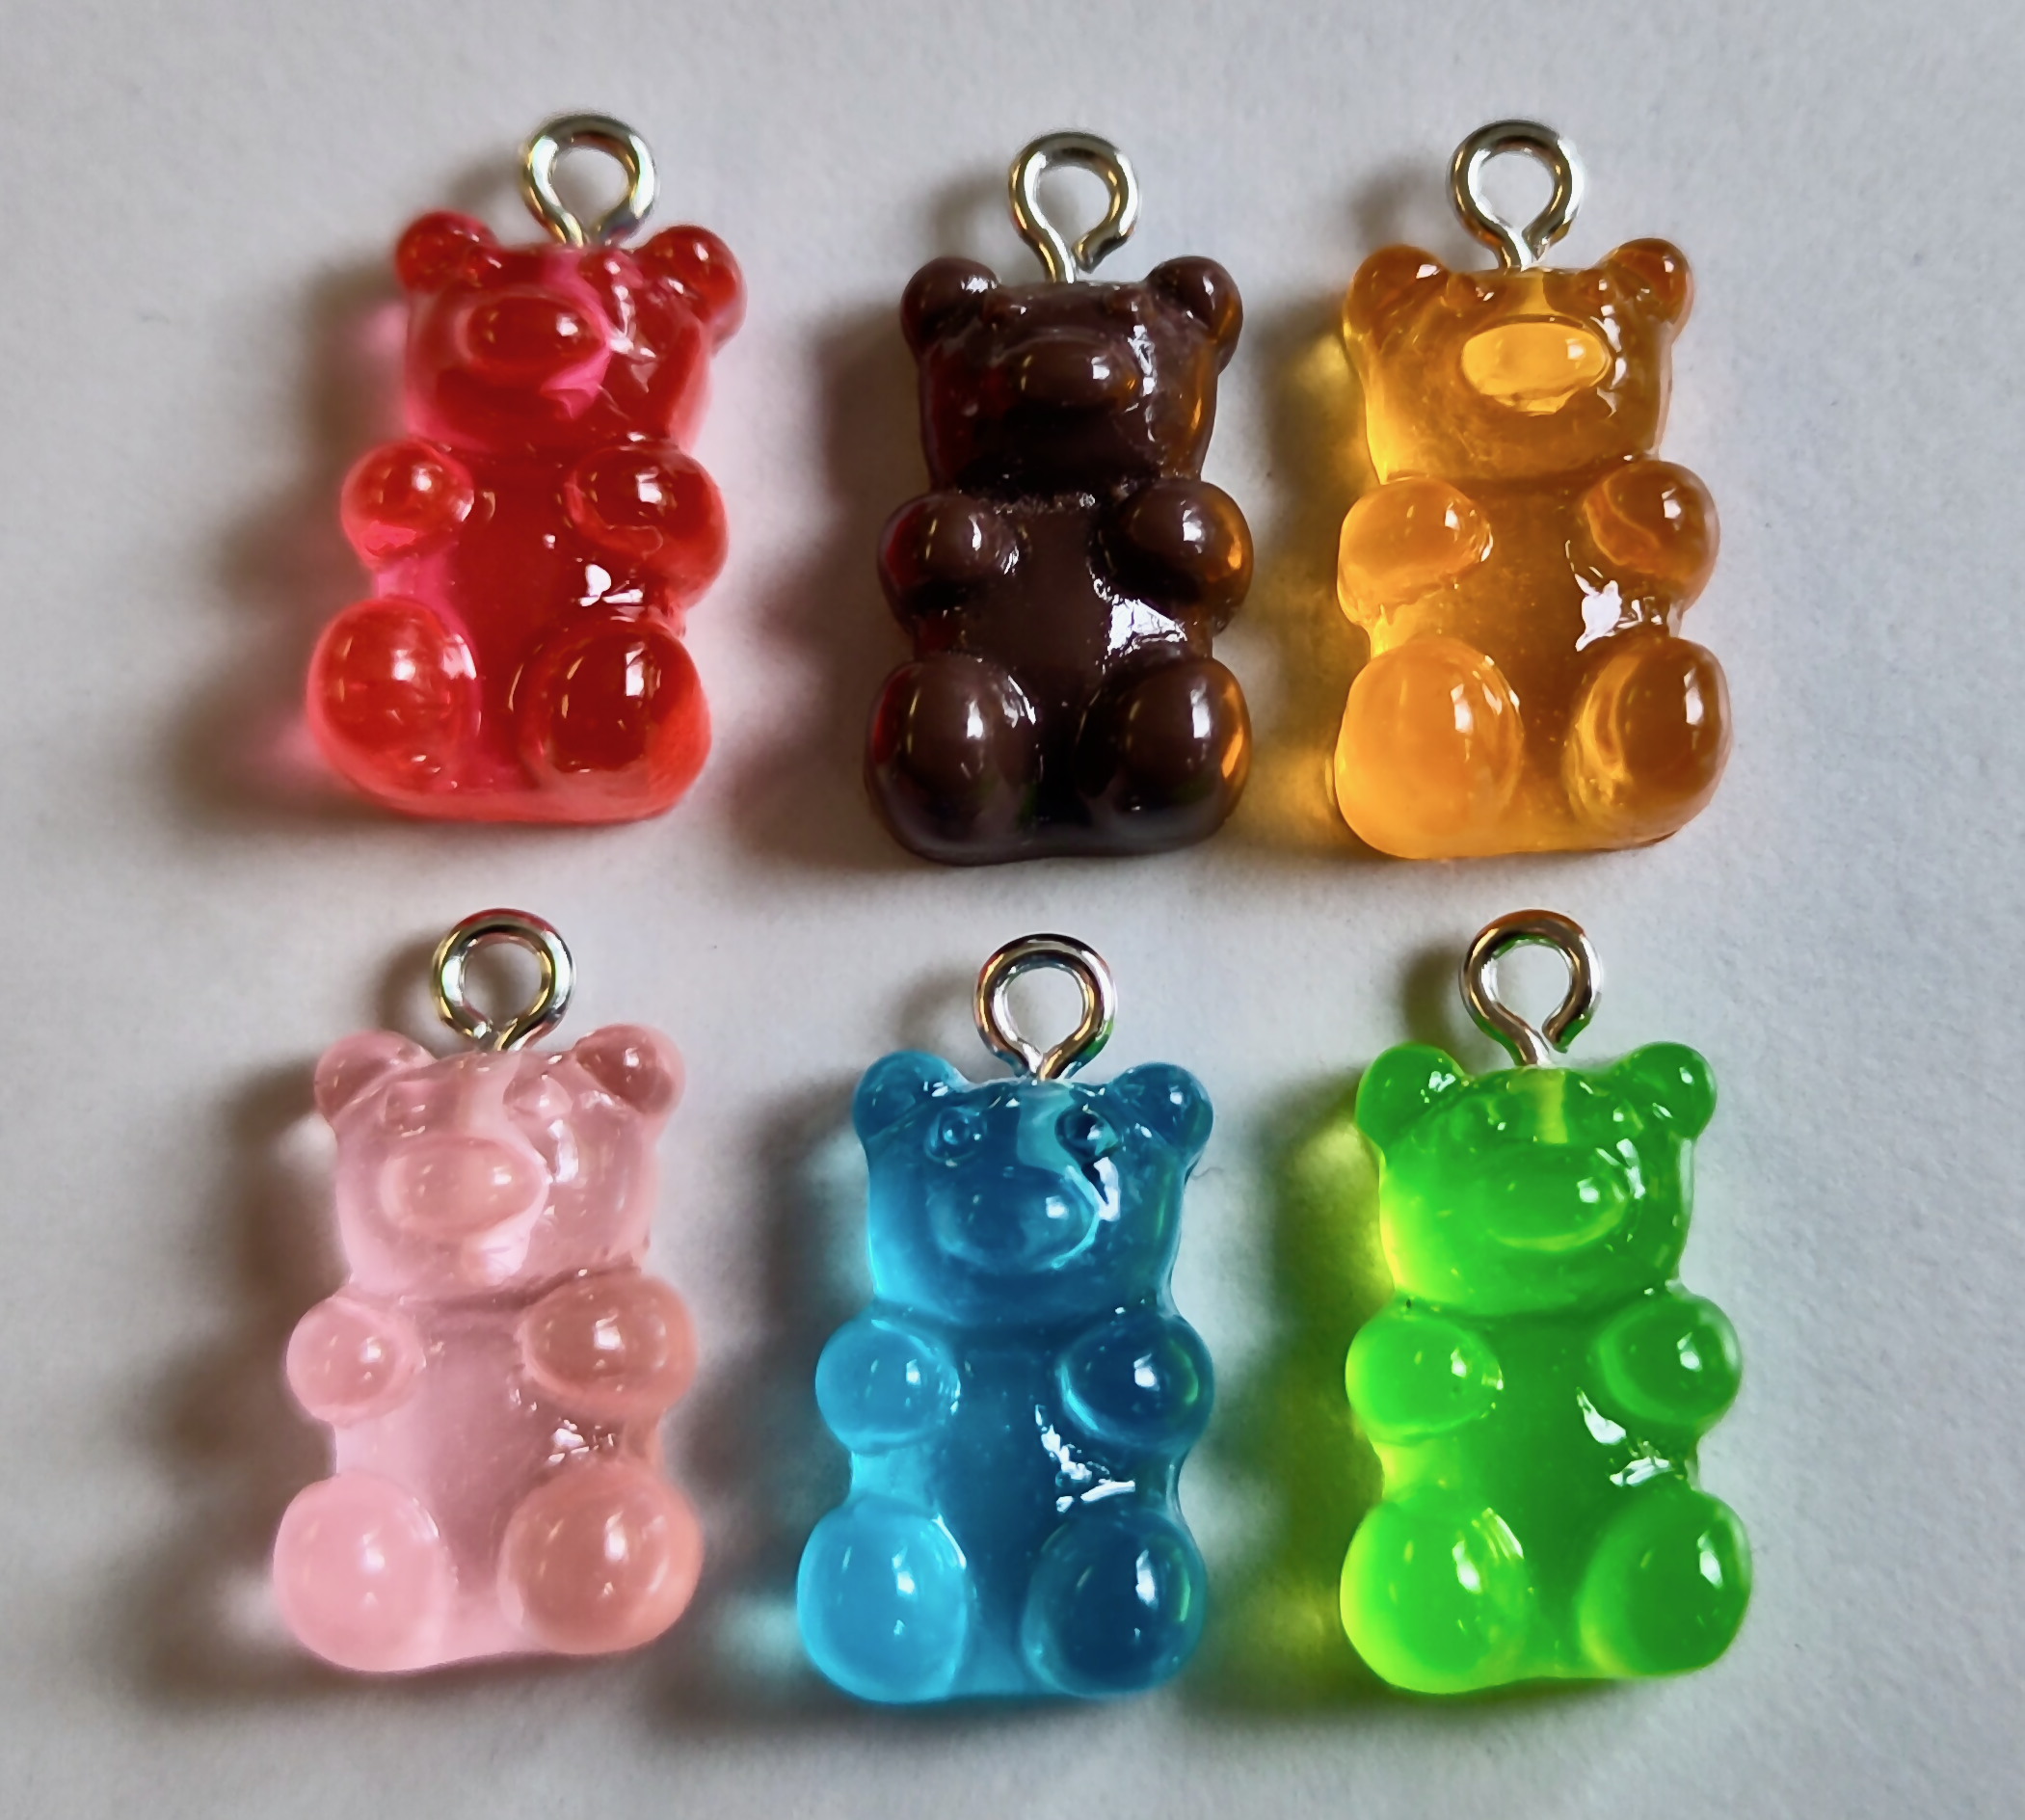
\includegraphics[width=0.25\textwidth]{images/storypoints.png}
\end{figure}

\section*{Aufbau}

\noindent Wir haben das Spielfeld bereits aufgebaut. Die Anleitung dazu ist unten. Prüft bitte, ob alles der Anleitung entspricht. Falls etwas anders sein sollte, gebt uns bitte Bescheid.

\begin{itemize}
    \item Sortiert die Events nach der Iteration. Die oberste Karte ist für Iteration 1, die unterste für Iteration 9. Legt sie so auf den Event-Stapel.
    \item Sucht die drei Features mit dem Start-Marker heraus und legt sie in den Backlog.
    \item Mischt die restlichen Features und legt sie auf den Feature-Stapel.
    \item Sucht den einen Bug mit dem Start-Marker heraus und legt ihn in den Backlog.
    \item Mischt die restlichen Bugs und legt sie auf den Bug-Stapel.
    \item Legt die 13 Technical Debt neben das Spielfeld.
    \item Legt sechs Storypoints in das Storypoint-Feld. Das ist bis auf weiteres euer dauerhaftes Kontingent.
    \item Legt die restlichen 14 Storypoints neben das Spielfeld.
\end{itemize}

\begin{figure}[H]
    \centering
    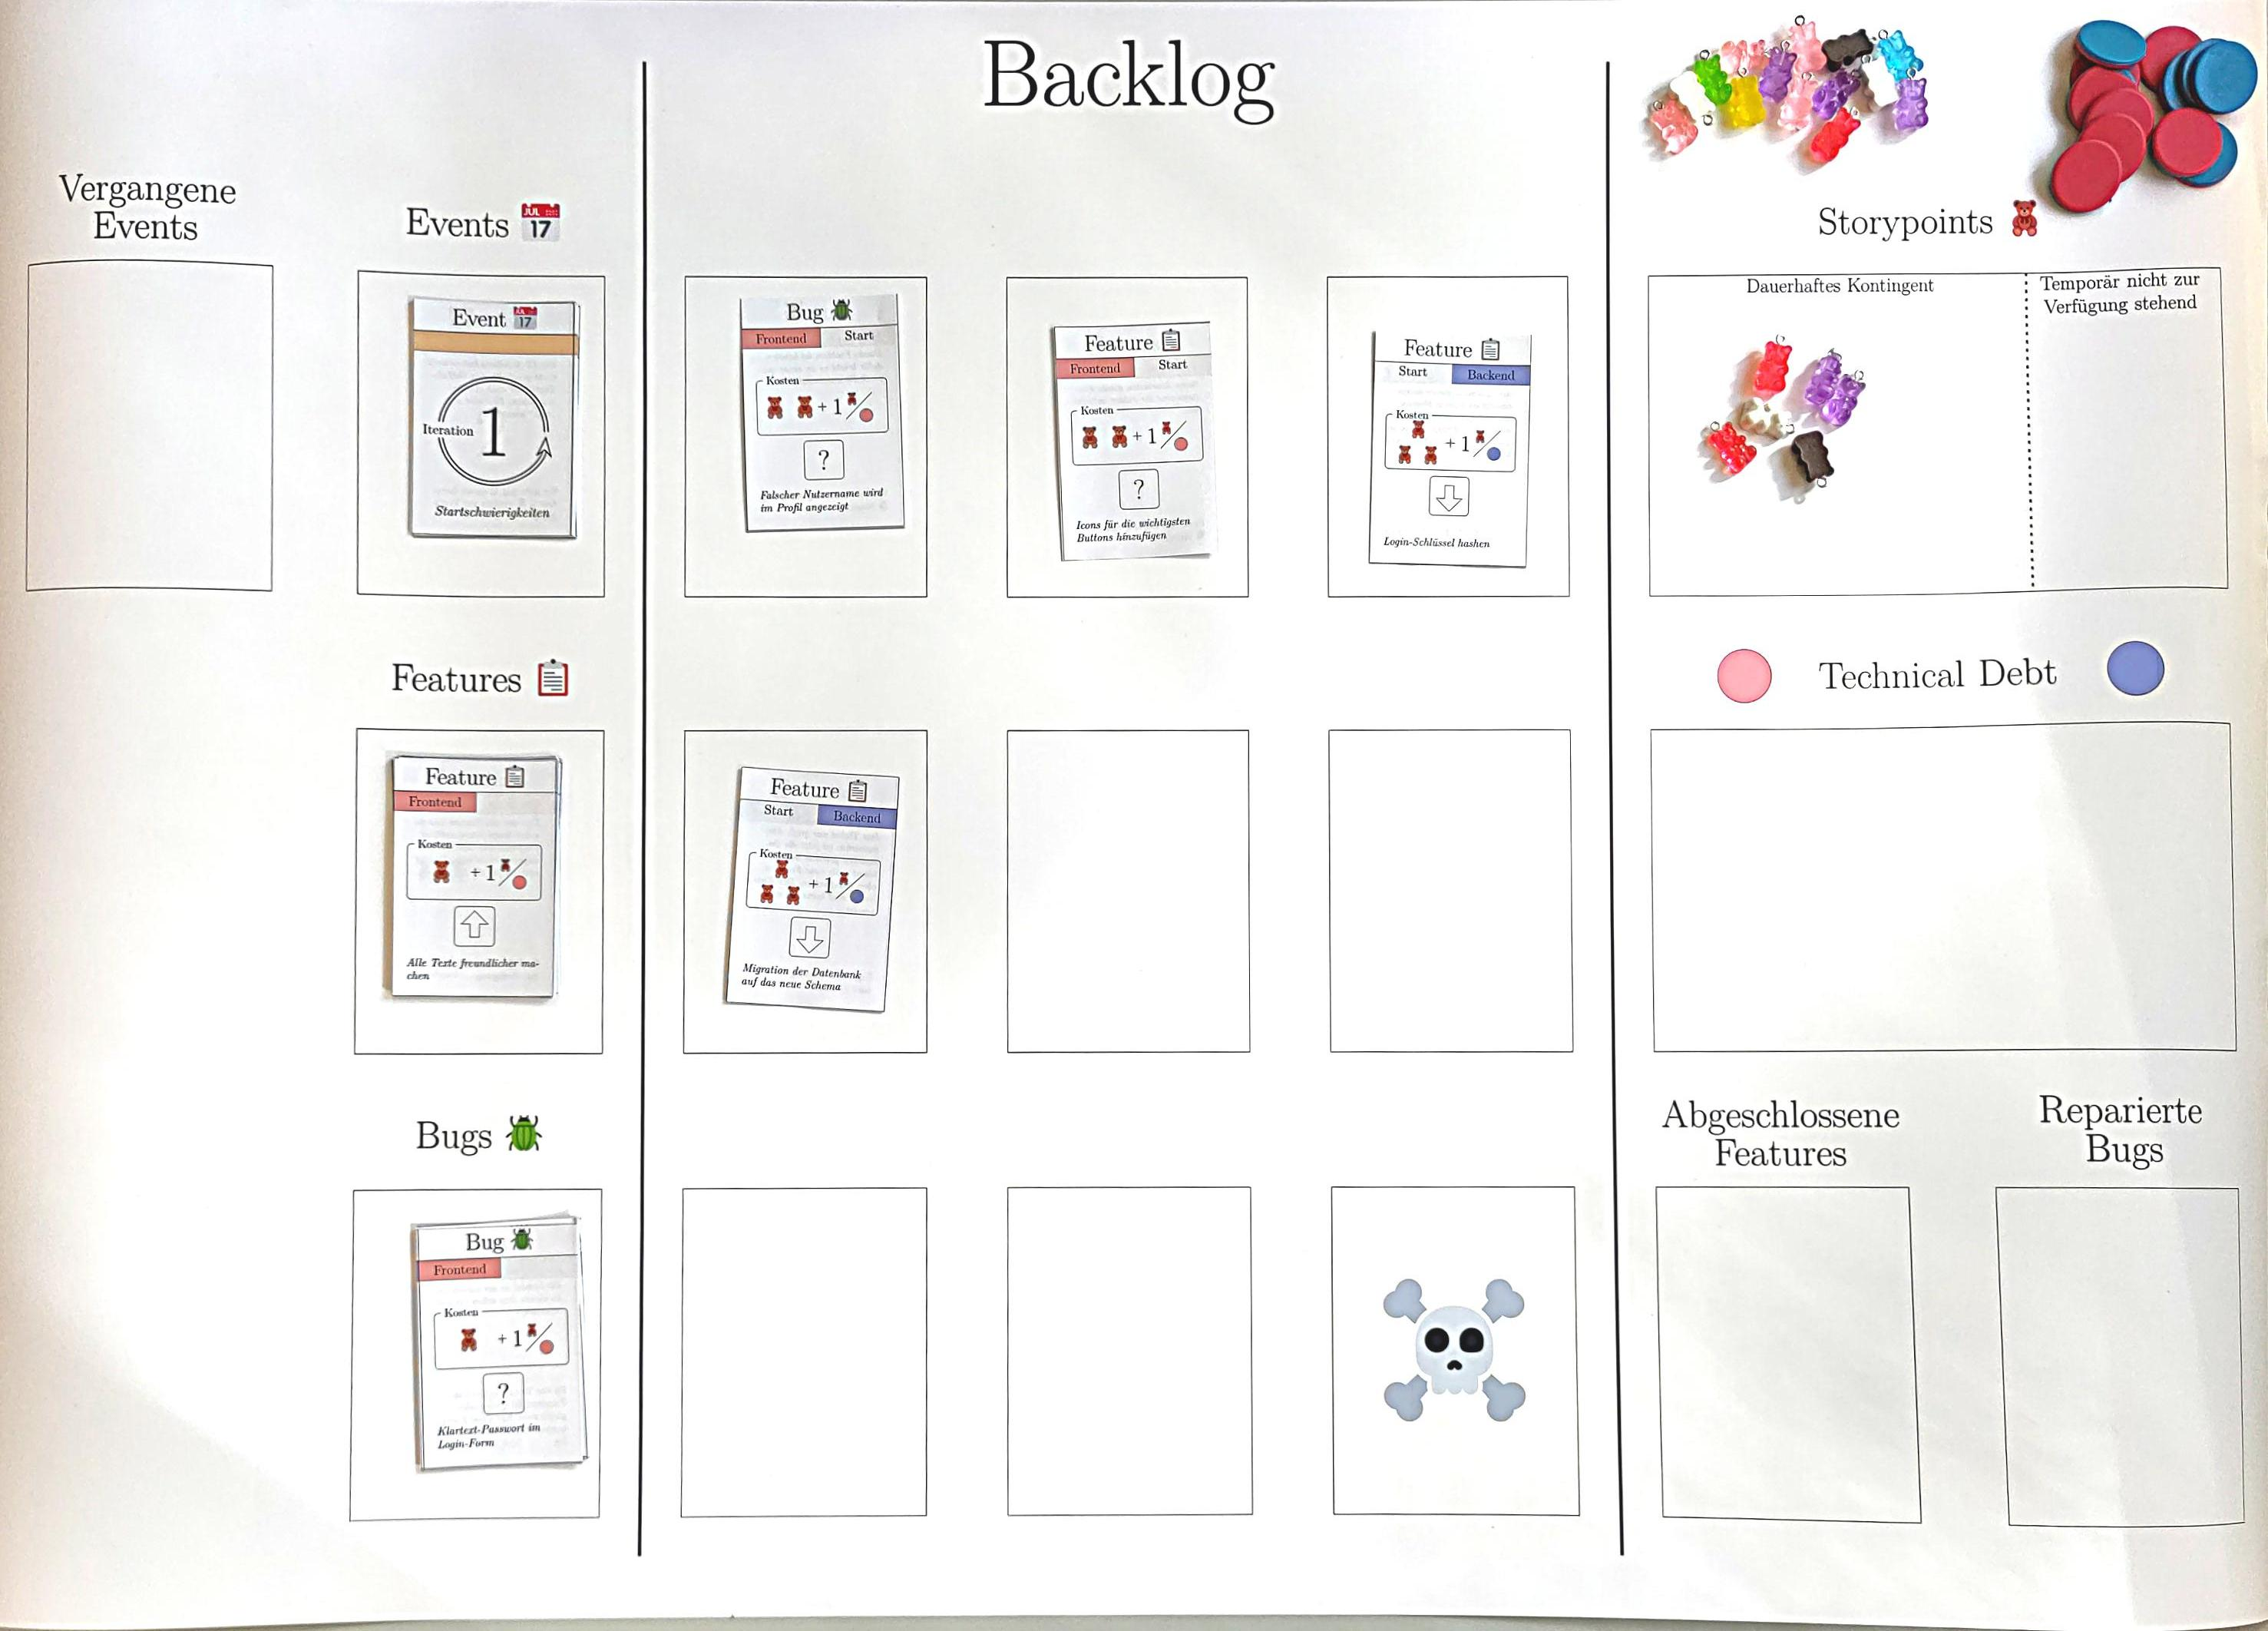
\includegraphics[width=\textwidth]{images/spielfeld_aufgebaut.jpg}
\end{figure}

\newpage

\section*{Spielablauf}

Das Spiel besteht aus aufeinander folgenden Runden bzw. Iterationen. Eine Iteration besteht aus folgenden Schritten:

\begin{enumerate}
    \item \textbf{Event}: Zieht die oberste Event-Karte, dreht sie um und führt den Effekt aus.
    \item \textbf{Feature nachziehen}: Nehmt das oberste Feature vom Feature-Stapel und legt es mit der Formel zur Kostenberechnung nach oben in den Backlog.
    \item \textbf{Planung der Iteration}: Wählt eine oder mehrere Aktionen für die Iteration aus. Ihr habt folgende Möglichkeiten:
    \begin{itemize}
        \item \textbf{Ticket(s) auswählen}: Wählt ein oder mehrere Tickets aus dem Backlog zur Bearbeitung aus. Legt dafür die Anzahl benötigter Storypoints auf das jeweilige Ticket. Die Anzahl benötigter Storypoints ist der feste Anteil vor dem Plus-Symbol, plus die Anzahl Technical Debt im zugehörigen Systemteil. \underline{Achtung}: wollt ihr in dieser Iteration im Frontend oder Backend refactorn, könnt ihr für diesen Systemteil kein Ticket aussuchen.
        \item \textbf{Abbau von Technical Debt / Refactoring}: Für jeden Technical Debt den ihr durch Refactoring entfernen wollt, müsst ihr einen Storypoint aufwenden. Legt den Storypoint auf den zu entfernenden Technical Debt. \underline{Achtung}: Falls ihr im Frontend refactort, könnt ihr in dieser Iteration keine Tickets im Frontend bearbeiten. Gleiches gilt für das Backend. Ihr könnt auch im Frontend und Backend gleichzeitig refactorn, dann dürfen aber keine Tickets bearbeitet werden.
        \item \textbf{Feature(s) nachziehen}: Nehmt ein oder mehrere Features vom Feature-Stapel und legt sie mit der Formel zur Kostenberechnung nach oben in den Backlog. Das kostet euch einen Storypoint pro nachgezogenem Feature.
    \end{itemize}
    \item \textbf{Ausführung der Iteration}: Arbeitet alles ab, was ihr diesen Sprint geplant habt:
    \begin{itemize}
        \item Entfernt den markierten Technical Debt
        \item Bearbeitet die ausgewählten Tickets, indem ihr sie umdreht, den Text lest und die Effekte ausführt. Die Reihenfolge ist euch überlassen.
    \end{itemize}
    \item \textbf{Technical Debt erhöhen}: Habt ihr in diesem Sprint mindestens ein Feature im Frontend bearbeitet, fügt genau einen Technical Debt im Frontend hinzu. Gleiches gilt für das Backend. Das Bearbeiten von Bugs führt nicht dazu, dass der Technical Debt erhöht wird.
    \item \textbf{Endbedingung prüfen}: Schaut, ob eine der Bedingungen für das Spielende erfüllt ist. Falls ja, endet das Spiel. Andernfalls bereitet die nächste Iteration vor.
    \item \textbf{Vorbereitung der nächsten Iteration}: Nehmt alle Storypoints die ihr für die Planung verwendet hat wieder auf das Storypoint-Feld. Achtung: Die Anzahl der verfügbaren Storypoints kann auch von Effekten beeinflusst werden. Manchmal stimmt das also nicht exakt überein. Die Effekte stellen das aber klar.
\end{enumerate}

\section*{Spielende und Punkte}

Das Spiel endet auf einem von zwei Wegen:

\begin{enumerate}
    \item Am Ende einer Iteration habt ihr neun oder mehr Tickets im Backlog. Das Projekt ist gescheitert. Ihr habt verloren.
    \item Ihr habt alle neun Iterationen abgeschlossen, ohne dass das Projekt gescheitert ist. Ihr habt gewonnen.
\end{enumerate}

\noindent Wenn ihr verloren habt, habt ihr 0 Punkte. Wenn ihr gewonnen habt, gibt jedes abgeschlossene Feature einen Punkt. Reparierte Bugs geben keine Punkte.

\end{document}
